\documentclass[12 pt]{article}
\usepackage[utf8]{inputenc}
\usepackage{a4}
\usepackage{indentfirst}
\usepackage{graphicx}
\usepackage{float}
\usepackage{tabularx}
\usepackage{multicol}
\usepackage{tikz, adjustbox}
\usepackage[most]{tcolorbox}
\usepackage{wrapfig}
\usepackage{amssymb}
\usepackage{hyperref}
\newcolumntype{M}[1]{>{\centering\arraybackslash}m{#1}}
\usepackage{titlesec}
\usepackage{listings}
\usepackage{xcolor}
\definecolor{codegreen}{rgb}{0,0.6,0}
\definecolor{codegray}{rgb}{0.5,0.5,0.5}
\definecolor{codepurple}{rgb}{0.58,0,0.82}
\definecolor{backcolour}{rgb}{0.95,0.95,0.92}
\emergencystretch=1em
\lstdefinestyle{mystyle}{
    backgroundcolor=\color{backcolour},  
    commentstyle=\color{codegreen},
    keywordstyle=\color{magenta},
    numberstyle=\tiny\color{codegray},
    stringstyle=\color{codepurple},
    basicstyle=\footnotesize\ttfamily,
    breakatwhitespace=false,         
    breaklines=true,                 
    captionpos=b,                    
    keepspaces=true,                 
    numbers=left,                    
    numbersep=5pt,                  
    showspaces=false,                
    showstringspaces=false,
    showtabs=false,                  
    tabsize=2,
    frame=single,
}
\lstset{style=mystyle}
% Yellow:
\definecolor{BgYellow}{HTML}{FFF59C}
\definecolor{FrameYellow}{HTML}{F7A600}
% Pink:
\definecolor{BgPink}{HTML}{EF6FA7}
\definecolor{FramePink}{HTML}{E5446E}


% Yellow Sticky Note (YStkyNote):
\newtcolorbox{YStkyNote}[1][]{%
    enhanced,
    before skip=2mm,after skip=2mm, 
    width=0.6\textwidth, % width of the sticky note
    boxrule=0.2mm,
    colback=BgYellow, colframe=FrameYellow, % Colors
    attach boxed title to top left={xshift=0cm,yshift*=0mm-\tcboxedtitleheight},
    varwidth boxed title*=-3cm,
    % The titlebox:
    boxed title style={frame code={%
        \path[left color=FrameYellow,right color=FrameYellow,
        middle color=FrameYellow]
        ([xshift=-0mm]frame.north west) -- ([xshift=0mm]frame.north east)
        [rounded corners=0mm]-- ([xshift=0mm,yshift=0mm]frame.north east)
        -- (frame.south east) -- (frame.south west)
        -- ([xshift=0mm,yshift=0mm]frame.north west)
        [sharp corners]-- cycle;
        },interior engine=empty,
    },
    sharp corners,rounded corners=southeast,arc is angular,arc=3mm,
    % The "folded paper" in the bottom right corner:
    underlay={%
        \path[fill=BgYellow!80!black] ([yshift=3mm]interior.south east)--++(-0.4,-0.1)--++(0.1,-0.2);
        \path[draw=FrameYellow,shorten <=-0.05mm,shorten >=-0.05mm,color=FrameYellow] ([yshift=3mm]interior.south east)--++(-0.4,-0.1)--++(0.1,-0.2);
        },
    drop fuzzy shadow, % Shadow
    fonttitle=\bfseries, 
    title={#1}
}
% Pink Sticky Note (PStkyNote):
\newtcolorbox{PStkyNote}[1][]{%
    enhanced,
    before skip=2mm,after skip=2mm, 
    width=0.4\textwidth, % width of the sticky note
    boxrule=0.2mm, 
    colback=BgPink, colframe=FramePink, % Colors
    attach boxed title to top left={xshift=0cm,yshift*=0mm-\tcboxedtitleheight},
    varwidth boxed title*=-3cm,
    % The titlebox:
    boxed title style={frame code={%
        \path[left color=FramePink,right color=FramePink,
        middle color=FramePink]
        ([xshift=-0mm]frame.north west) -- ([xshift=0mm]frame.north east)
        [rounded corners=0mm]-- ([xshift=0mm,yshift=0mm]frame.north east)
        -- (frame.south east) -- (frame.south west)
        -- ([xshift=0mm,yshift=0mm]frame.north west)
        [sharp corners]-- cycle;
        },interior engine=empty,
    },
    sharp corners,rounded corners=southeast,arc is angular,arc=3mm,
    % The "folded paper" in the bottom right corner:
    underlay={%
        \path[fill=BgPink!80!black] ([yshift=3mm]interior.south east)--++(-0.4,-0.1)--++(0.1,-0.2);
        \path[draw=FramePink,shorten <=-0.05mm,shorten >=-0.05mm,color=FramePink] ([yshift=3mm]interior.south east)--++(-0.4,-0.1)--++(0.1,-0.2);
        },
    drop fuzzy shadow, % Shadow
    fonttitle=\bfseries, 
    title={#1}
}
\title{\huge{Lecture Notes 2: PLD}}
\author{}
\date{}
\begin{document}
\maketitle
\tableofcontents
\newpage

\section{Overview}
PLD stands for Programmable Logic Device, and it can be classified into:
\begin{itemize}
    \item \textbf{ROM:} \begin{itemize}
        \item Consists of OR gates and a decoder
        \item Programmable OR gates and fixed AND gates
        \item if I have n inputs, then I need $2^n$ AND gates
        \item OR gates are programmed using fuses.
    \end{itemize}
    \item \textbf{PLA (Programmable Logic Array):}\begin{itemize}
        \item Programmable AND gates
        \item Programmable OR gates (using fues)
        \item Slower compared to PAL
    \end{itemize} 
    \item \textbf{PAL (Programmable Array Logic):}\begin{itemize}
        \item Programmable AND gates
        \item Fixed OR gates
    \end{itemize}
    \item \textbf{FPGA (Field Programmable Gate Array)}
\end{itemize}
\section{Implement using PLA}
$f_1=AB`+AC+A`BC`$

$f_2=(AC+AB)`$
\begin{figure}[H]
    \centering
    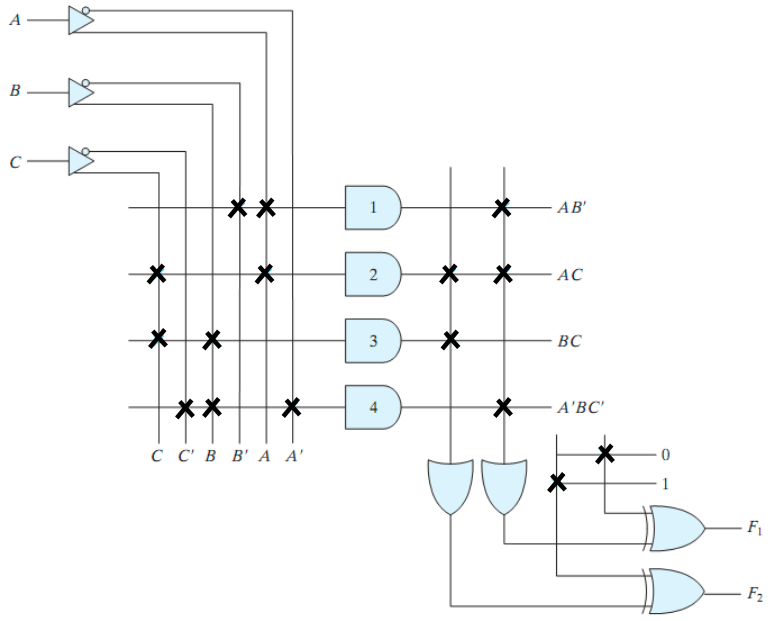
\includegraphics[scale=0.3]{./images/micro1}
    \label{micro1} 
\end{figure}
Using XOR at the end to allow a complement output
\section{PAL}
\subsection{PAL chips}
\begin{minipage}{8cm}
\textbf{Examples}
\begin{itemize}
    \item \textbf{16L8:} \begin{itemize}
        \item up to 16 inputs
        \item up to 8 outputs
        \item active low
    \end{itemize}
    \item \textbf{16H8:} active high
    \item \textbf{16R8:} uses register
    \item \textbf{16A8:} arithmetic (uses XOR)
\end{itemize}
\end{minipage}
\hfill
\begin{minipage}{10cm}
\begin{YStkyNote}[Note 1]
    16 and 8 aren't constants, they are just used as examples
\end{YStkyNote}
\end{minipage}
\subsection{GAL chips}
\textbf{GAL (Generic Array Logic):} It contains a macro-cell, which allows you to control whether your PAL should act as (L),(H),(R),(A)
\begin{figure}[H]
    \centering
    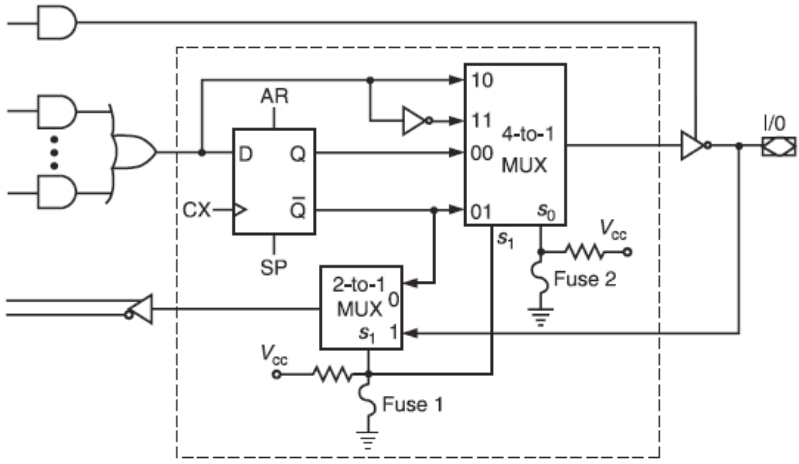
\includegraphics[scale=0.4]{./images/micro2}
    \label{micro2} 
\end{figure}
\begin{itemize}
    \item \textbf{To act as R:} using the D flip-flop
    \item \textbf{To act as L or H:} using (10), (11) in the 4 to 1 MUX
    \item \textbf{The 2 to 1 MUX}: To allow a feedback from the function, or to use the output as an input
\end{itemize}
\subsection{Implement using PAL}

$W=ABC`+A`B`CD`$

$X = A + B C D$

$Y = A` B +C D + B` D`$

$Z = W + A C` D` +A` B` C` D$
\begin{figure}[H]
    \centering
    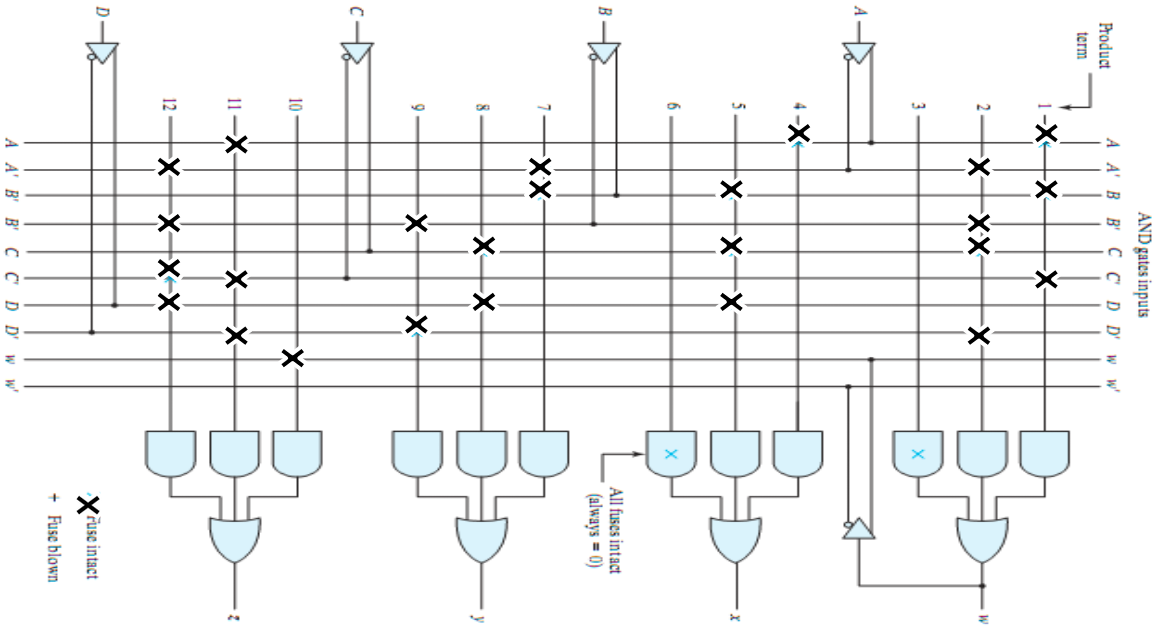
\includegraphics[scale=0.35]{./images/micro3}
    \label{micro3} 
\end{figure}
\section{FPGA}
\begin{itemize}
    \item \textbf{CLB (Configurable Logic Block):} Implement combinatorial and sequential logic Based on LUT and DFF 
    \begin{figure}[H]
    \centering
    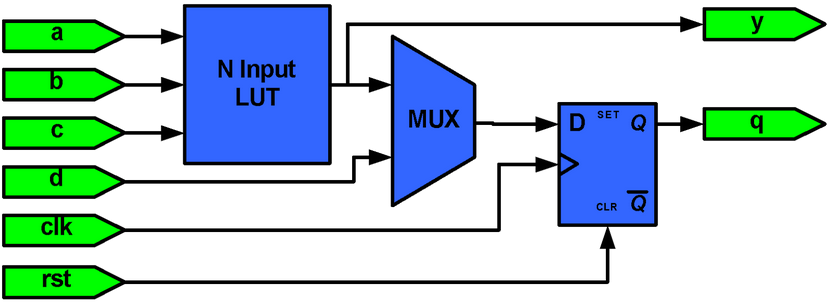
\includegraphics[scale=0.33]{./images/micro4}
    \label{micro4} 
\end{figure}
\item \textbf{Programmable I/O blocks (IOB):}\begin{itemize}
    \item Configurable I/Os for external connections.
    \item Supports various voltages and tri-states
\end{itemize}
\item \textbf{Programmable Interconnects}\begin{itemize}
    \item Switches
    \item Horizontal/vertical lines
    \item allow logic blocks to be connected to each other and to the I/O pins
\end{itemize}
\end{itemize}

\subsection*{LUT}
\textbf{LUT:} A ram with width of 1 bit
    \begin{figure}[H]
    \centering
    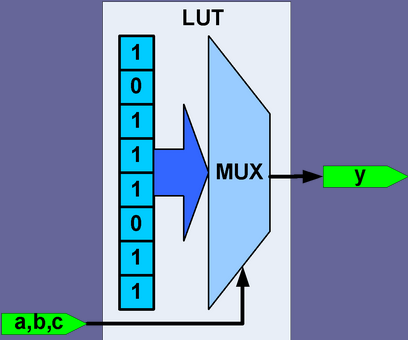
\includegraphics[scale=0.4]{./images/micro5}
    \label{micro5} 
\end{figure}
\begin{itemize}
    \item \textbf{Block of bits entering the MUX:}It's a register that contains the truth table of each function
    \item\textbf{Number of functions:} It can represent $2^n$ functions, where n is the number of bits in each register.
\end{itemize}

\end{document}
